\documentclass[12pt]{article}
\usepackage[utf8x]{inputenc}
\usepackage[english,russian]{babel}
\usepackage[section]{placeins}
\usepackage{upgreek}
\usepackage{graphicx}
\usepackage[left=3cm, right=1.5cm, top=2cm, bottom=2cm]{geometry}
\usepackage{caption}
\usepackage{subcaption}
\usepackage{indentfirst}
\usepackage{wrapfig}
\usepackage{amsmath}
\usepackage{gensymb}
\usepackage{setspace}
\usepackage{placeins}
\graphicspath{{images/}}

% \textheight 24.5cm % 29.7-2-2=25.7
% \textwidth 17cm % 21-2.5-1.5=17.0
% \hoffset -0.04cm %2.5-2.54=-0.04 слева 3см
% \voffset -0.54cm %2-2.54=0.54 сверху 2см
% \oddsidemargin 0cm
% \headheight 0cm
% \headsep 0cm
% \topmargin 0cm
\onehalfspacing

% \textheight 25.7cm % 29.7-2-2=25.7
% \textwidth 17cm % 21-2.5-1.5=17.0
% \hoffset -0.04cm %2.5-2.54=-0.04 слева 3см
% \voffset -1.04cm %2-2.54=0.54 сверху 2см
% \oddsidemargin 0cm
% \headheight 0cm
% \headsep 0cm
% \topmargin 0cm
% \setcounter{page}{1}
\def\sigspace{\\[1em]
\underline{\hspace{5cm}}\\[-0.2em]}

\def\etal{{et~al.}}

\begin{document}

\begin{titlepage}
	\begin{center}
		{
		{\bf Санкт-Петербургский Государственный Университет\\
		\vskip 1em
		Астрономия\\
		Теоретическая астрофизика} }

	\vspace{3cm}
  	
	{\large Дмитриев Денис Витальевич}
  
  \vskip 2em
  

	\Large{\bf{Магнитосферная аккреция на медленно вращающиеся молодые звезды}}
  \vskip 1em
  {\normalsize {Дипломная работа}\\}
	\end{center}
	
	\vskip 5em
  
	{
		 \begin{flushright}
			\textbf{Научный руководитель:}\\
		  д.ф.-м.н, профессор, В.П.\,Гринин \\
		  \bigskip
		  \textbf{Рецензент:}\\
		  д.ф.-м.н, Л.В. Тамбовцева \sigspace
		 \end{flushright}
	}

	\vfill
	\begin{center}
	\small {Санкт-Петербург

	2018}
	\end{center}
\end{titlepage}

\newpage


\begin{titlepage}
	\begin{center}
		{
		{\bf Saint-Petersburg State University\\
		\vskip 1em
		Astronomy\\
		Theoretical astrophysics} }

	\vspace{3cm}
  	
	{\large Denis Dmitriev}
  
  \vskip 2em
  

	\Large{\bf{Magnetospheric accretion on slowly rotating young stars}}
  \vskip 1em

  {\normalsize {Graduation Thesis}\\}
	\end{center}
	
	\vskip 5em
  
	{
		 \begin{flushright}
			\textbf{Scientific supervisor:}\\
		  Doctor of Physics and Mathematics, \\ Professor V.P. Grinin \\
		  \bigskip
		  \textbf{Reviewer:}\\
		  Doctor of Physics and Mathematics, \\ L.V. Tambovtseva\sigspace
		\end {flushright}
	}

	\vfill
	\begin{center}
	\small {Saint-Petersburg

	2018}
	\end{center}
\end{titlepage}

\newpage
\tableofcontents
\newpage


% \begin{abstract}

% Рассматривается образование эмиссионных линий водорода в магнитосферах молодых звезд. Предполагается, что магнитосфера образована дипольным магнитным полем, ось которого совпадает с осью вращения звезды. Перенос излучения в спектральных линиях рассматривается в приближении Соболева с учетом нелокального радиационного взаимодействия. Распределение плотности и температуры газа в магнитосфере принято таким же, как в работе Хартманна и др., 1994 \cite{hartmann94}. Приведены результаты расчетов интенсивностей и профилей линий $H_\alpha$, $H_\beta$, $H_\gamma$ и линии $Br_\gamma$ для случая медленно вращающейся звезды. Отдельно рассмотрена модель магнитосферы, в которой падающий газ нагревается излучением аккреционого пятна на поверхности звезды.

% \end{abstract}

\section{Введение}


Данная работа посвящена разработке модели аккреции водородного газа на медленно вращающиеся молодые звезды. Можно сказать, что рассматриваются звезды типа Т Тельца, так как их скорости вращения сравнительно малы (в среднем около 15 км/с на экваторе) \cite{petrov03}.

Тип T Тельца --- это звезды, еще не достигшие главной последовательности. Звезды этого типа имеют среднюю температуру около 4000 K и массы в интервале от 0.2 до 2 $M_\odot$ \cite{petrov03}. Многие молодые звезды окружены околозвездными газопылевыми дисками, в которых формируются планетные системы. Вещество дисков аккрецирует на звезды. Важную роль в этом процессе играет крупномасштабное магнитное поле молодой звезды (см. например, Хартманн и др. 1994 года \cite{hartmann94}). У звезд типа Т Тельца оно достигает значений порядка 1-2 кГс \cite{petrov03}.

Считается, что сильное магнитное поле звезды захватывает аккрецирующий газ, нарушая кеплеровский диск, и падение на звезду происходит не на экваторе, а на высоких широтах. Такая модель позволяет объяснить низкую скорость вращения звезд типа Т Тельца и характерные профили линий. При этом избыточный момент импульса уносится дисковыми ветрами, образующимся при аккреции \cite{matt05}. Модель магнитосферы была впервые рассмотрена в работе Хартманна и др. 1994 года \cite{hartmann94} и впоследствии усовершенствована в работах Мацеролле и др. 2001 года \cite{muzerolle01} и Лима и др. 2010 года \cite{lima10}.

В данной работе описывается модель, разработанная с помощью цитируемых выше работ, с помощью которой можно рассчитывать профили магнитосферных линий. Рассматривается водородный газ, вмороженный в дипольное магнитное поле звезды. Поскольку скорости движения газа в магнитосфере значительно больше тепловых, можно использовать приближение Соболева для решения системы уравнений стационарности. Однако, нужно также учесть нелокальное радиационное взаимодействие, возникающее между областями магнитосферы, лучевая скорость которых относительно друг-друга равна нулю. Такая задача впервые была рассмотрена в работе Грачева и Гринина 1975 года \cite{grachev75}, а позже боле детально в работе Райбики и Хаммера 1978 года \cite{rybicki78}. 

\begin{figure}[h] 
\centering
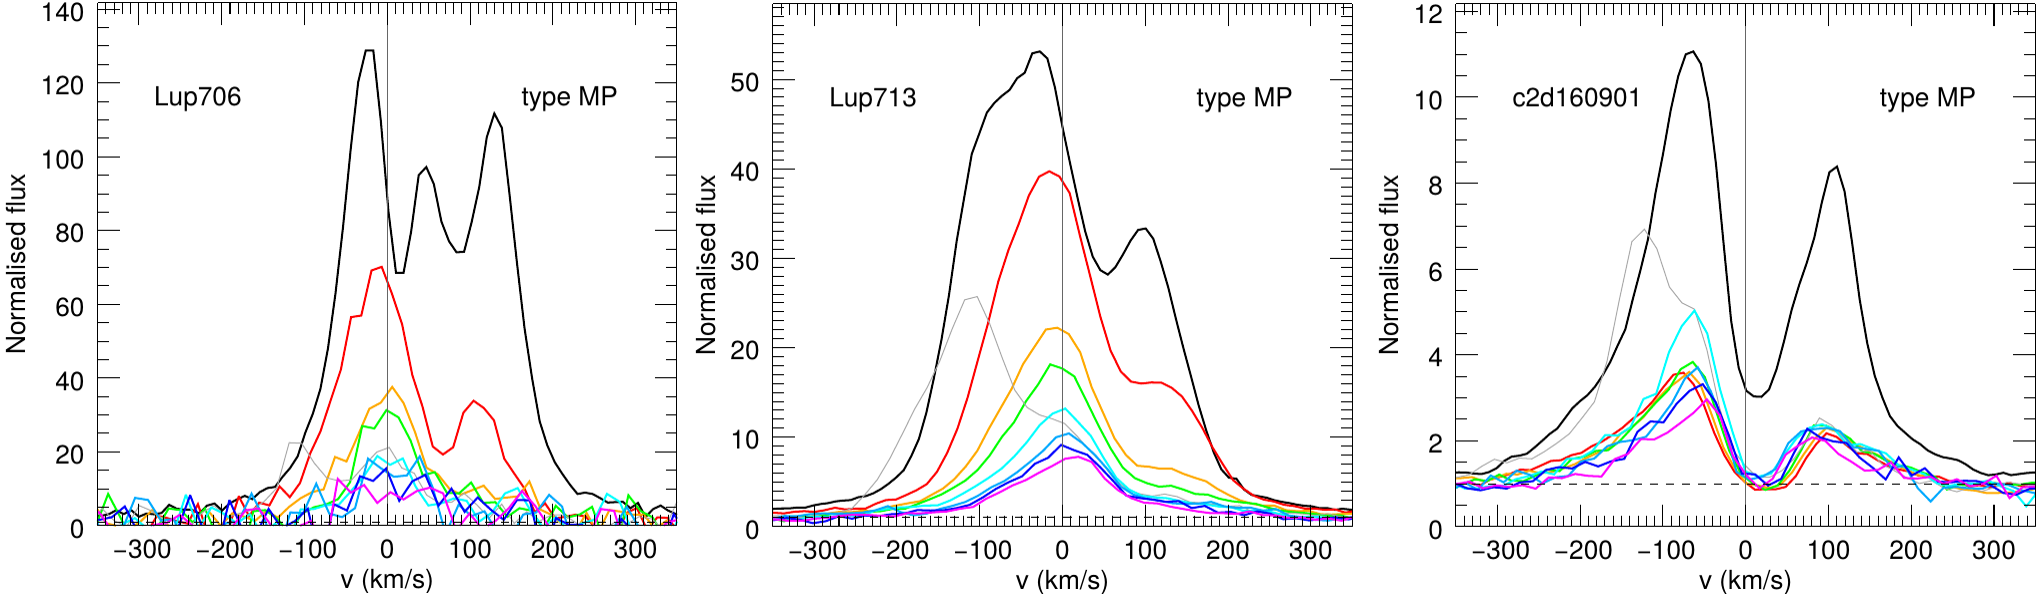
\includegraphics[width=\textwidth]{profiles.png}
\caption{Профили водородных линий из \cite{antoniucci17}, наблюдающиеся в спектрах различных молодых звезд. Показаны линии $\text{H}\alpha$ (черный), $\text{H}\beta$ (красный), $\text{H}\gamma$ (оранжевый), $\text{H}\delta$ (зеленый), H8 (циан), H9 (бирюзовый), H10 (синий), H11 (фуксин). H7 показана серым, так как она блендируется с линией CaII. }
\label{fig:profiles}
\end{figure}

Мы во многом повторяем результаты, полученные в статьях Хартманна и др. \cite{hartmann94} и Мацеролле и др. \cite{muzerolle01}, однако вносим некоторые модернизации в их модель, учитывающие современные представления о физике процесса. В частности, рассматривается модель аккреции на наклонный диполь, которая в указанных выше работах не рассматривалась. Подобная модель необходима для понимания формирования профилей линий в спектрах молодых звезд. В дальнейшем предполагается подключить магнитосферную модель к уже имеющимся ветровым моделям \cite{tambovtseva14}, \cite{grinin11}, чтобы получить инструмент, позволяющий детально моделировать эмиссионные спектры молодых звезд. Примеры различных профилей бальмеровских линий в спектрах звезд типа Т Тельца из статьи \cite{antoniucci17} показаны на рис. \ref{fig:profiles}.

Мы рассчитываем состояния возбуждения водорода для канонической модели соосной (с осью вращения) магнитосферы, однако при расчете профилей мы оставляем возможность отклонять магнитосферу от оси вращения на небольшой угол, при котором форма магнитосферы еще не сильно меняется. Отклонением оси магнитосферы от оси вращения часто объясняют вращательную модуляцию профилей линий (см. например \cite{bouvier99}, \cite{petrov01}).

\section{Cостояние газа в магнитосфере}

Мы предполагаем, что звезда имеет настолько сильное магнитное поле, что падающий газ полностью вморожен в него. Также мы считаем, что газ не возмущает магнитное поле, которое предполагается дипольным. Соответственно линии тока газа задаются уравнением силовых линий поля

\begin{equation} \label{eq:dipole}
r = r_\text{m} \sin^2 \theta,
\end{equation}
где $\theta$ --- полярный угол от оси симметрии, $r$ --- расстояние до звезды, а расстояние $r_\text{m}$ соответствует $\theta = \pi/2$. Следуя работе Хартманна и др. \cite{hartmann94}, предполагаем, что существует внешняя и внутренняя граница магнитосферы: $r_\text{mo}$ и $r_\text{mi}$, и газ течет только по линиям тока с $r_\text{mi} < r_\text{m} < r_\text{mo}$. Ниже мы будем использовать сферическую систему координат с началом отсчета в центре звезды и осью сонаправленной с осью симметрии. Выбор сферической системы координат обусловлен тем, что для решения задачи переноса излучения направление на звезду является выделенным, как и в принятой системе координат.

Предполагая, что газ падает на звезду с расстояния $r_\text{m}$ только под действием силы тяготения, вычисляем модуль скорости его падения

\begin{equation} \label{eq:velabs}
|\vec{v}| = v_\text{esc}\sqrt{\left(\frac{R_\star}{r} - \frac{R_\star}{r_\text{m}}\right)},
\end{equation}
где $v_\text{esc}$ --- скорость убегания с поверхности звезды. Так как газ движется вдоль силовых линий, а величина скорости задается \eqref{eq:velabs}, можно записать вектор скорости в сферической системе координат

\begin{align} \label{eq:velvec}
 \vec{v} & = v \hat{r} + u \hat{\theta}/r, \\
 v & = -2v_\text{esc}\sqrt{\frac{R_\star}{r}}\frac{\cos^2\theta}{\sqrt{4-3y}}, \nonumber \\
 u & = -v_\text{esc}\sqrt{\frac{R_\star}{r}}\frac{\cos\theta\sin\theta}{\sqrt{4-3y}}, \nonumber
\end{align}
где $y = \sin^2\theta = r/r_\text{m}$, a $\hat{r}$, $\hat{\theta}$ и отсутствующий в этом соотношении $\hat{\phi}$ это базисные вектора сферической системы координат. Компонента скорости при $\hat{\phi}$ равна нулю, так как мы предполагаем, что магнитосфера вращается твердотельно, а значит для решения задачи переноса излучения можно считать что вращения нет.

Ход плотности и температуры в магнитосфере мы заимствуем из работы Хартманна 1994 года \cite{hartmann94}, но вносим дополнительный экспоненциально затухающий член в ход температуры

\begin{equation} \label{eq:temp}
 T = T_{\text{hart}} + T_\text{hot}\exp\left(-\frac{r - R_\star}{d_\text{hot} R_\star}\right)
\end{equation}

Такой дополнительный член должен привести к появлению дополнительной эмиссии в спектральных линиях (Додин \cite{dodin18}). Он обусловлен тем, что горячее аккреционное пятно, образующееся за фронтом ударной волны в результате перехода кинетической энергии падающего газа в тепловую (Ламзин \cite{lamzin98}),
 %температура которого может достигать 10-20 тысяч кельвинов \cite{dodin18},
 может нагревать падающий газ у поверхности звезды \cite{dodin18}.

% В моделях Хартманна и др. также учитывается вклад излучения горячего пятна: создается дополнительный континуум, который влияет на всю магнитосферу. Однако мы считаем, что это излучение должно очень быстро поглотится в сравнительно тонком слое рядом с поверхностью звезды, так как магнитосфера оптически толстая, поэтому не учитываем излучение этого пятна.

\section{Уравнения стационарности. Учет нелокального радиационного взаимодействия}

Система уравнений стационарности для атома водорода взята из статьи \cite{katysheva80} и имеет вид

 
\begin{align} \label{eq:stat}
n_i & \left[ \sum\limits_{j=1}^{i-1} (A_{ij} + B_{ij}J_{ij}) + \sum\limits_{k=i+1}^\infty B_{ik}J_{ik} + n_e ( q_{ic} + \sum\limits_{j \neq i}^\infty q_{ij} ) + B_{ic}WJ_{ic}^\star \right] = \nonumber \\
 & \sum\limits_{k=i+1}^\infty n_k (A_{ki} + B_{ki}J_{ki}) + \sum\limits_{j=1}^{i-1} n_jB_{ji}J_{ij} + \nonumber \\
 & n_e \sum\limits_{j\neq i}^\infty n_jq_{ji} + n_en^+C_i + n_e^2n^+Q_{ci} \\
 & i=1,\ 2,\ ... \nonumber
\end{align}

Здесь $n_i$ --- населенность i-го уровня, $n_e$, $n^+$ --- концентрация электронов и протонов (так как газ водородный $n_e = n^+$), $q_{ik}$ --- коэффициенты ударного взаимодействия и ионизации, $Q_{ci}$ --- коэффициент тройной рекомбинации, $C_i$ и $B_{ic}$ --- коэффициенты фоторекомбинации и ионизации с учетом вынужденных переходов, а $J_{ik}$ --- средняя интенсивность в линии перехода $i\rightarrow k$.  

\begin{figure}[h]
\centering
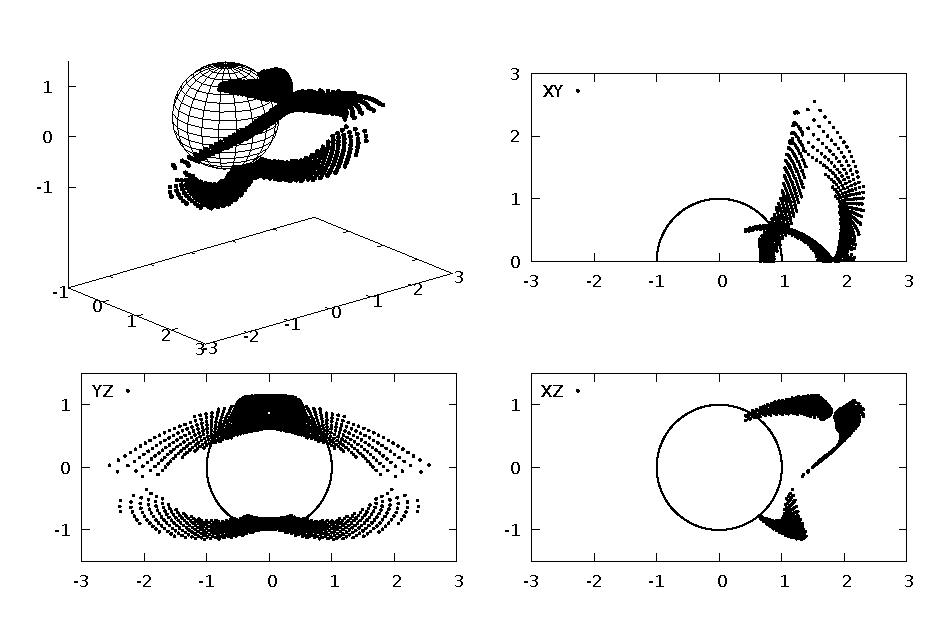
\includegraphics[width=0.9\textwidth]{surf.eps}
\caption{СР-поверхность в магнитосфере с $r_\text{mi} = 2.2$ и $r_\text{mo} = 3.0$ для точки с координатами $r_\text{m} = 2.4\ R_\star$, $\theta = 65\degree$ ($\text{X,Y,Z} = 1.8,0,0.8$). Слева сверху показан 3D вид поверхности, сферой нарисована поверхность звезды. Справа сверху, слева снизу и справа снизу --- проекции на три координатных плоскости, на которых окружностью также нарисована поверхность звезды.}
\label{fig:CPsurf}
\end{figure}

Для расчета средней интенсивности излучения в линии мы используем приближение Соболева с учетом нелокального радиационного взаимодействия. Метод впервые был описан в работе \cite{grachev75}, а затем более подробно в работе \cite{rybicki78}. Нелокальное взаимодействие возникает из-за того, что лучевая скорость некоторых областей магнитосферы относительно друг-друга равна нулю (т. е. точки не удаляются и не приближаются). В таком случае излученный в одной точке магнитосферы фотон может поглотиться в другой, достаточно удаленной точке. Множество, образуемое всеми взаимодействующими таким образом точками с некоторой фиксированной точкой, называют CP-поверхностью (common point) или s-поверхностью. Вид CP-поверхности в магнитосфере показан на рис. \ref{fig:CPsurf}. Средняя интенсивность в таком случае записывается как
\FloatBarrier
\begin{equation} \label{eq:meanint}
J_{ki} = (1-\beta_{ik}(\vec{r}))S_{ki}(\vec{r}) + \beta_{ik}^\star(\vec{r})I^\star_{ki} + F_{ki}(\vec{r}),
\end{equation}
где $S_{ki}$ --- функция источника в линии:
\begin{equation} \label{eq:source}
S_{ki} = \frac{2h\nu_{ki}^3}{c^2}\left( \frac{n_i}{n_k} \frac{g_k}{g_i} - 1 \right)^{-1},
\end{equation}
$\beta_{ik}(\vec{r})$ --- средняя вероятность выхода кванта в произвольном направлении без рассеяний:
\begin{equation} \label{eq:beta}
\beta_{ik}(\vec{r}) = \frac{1}{4\pi}\int\limits_{(4\pi)} d\Omega(\vec{n})\frac{1-e^{\tau_{ik}(\vec{r},\vec{n})}}{\tau_{ik}(\vec{r},\vec{n})}, 
\end{equation}

\begin{equation} \label{eq:starbeta}
\beta_{ik}^\star(\vec{r}) = \frac{1}{4\pi}\int\limits_{\Omega_\star} d\Omega(\vec{n})\frac{1-e^{\tau_{ik}(\vec{r},\vec{n})}}{\tau(\vec{r},\vec{n})}e^{-\sum_{j=1}^N\tau_{ik}(\vec{r_j},\vec{n})},
\end{equation}

\begin{equation} \label{eq:CPF}
F_{ki}(\vec{r}) = \frac{1}{4\pi}\int\limits_{(4\pi)} d\Omega(\vec{n})\frac{1-e^{\tau_{ik}(\vec{r},\vec{n})}}{\tau(\vec{r},\vec{n})}\sum\limits_{j=1}^N S_{ki}(\vec{r_j}) (1-e^{\tau_{ik}(\vec{r_j},\vec{n})}) e^{-\sum_{i=1}^{j-1}\tau_{ik}(\vec{r_j},\vec{n})}),
\end{equation}
где $F_{ki}$ учитывает нелокальное взаимодействие, $\vec{n}$ --- вектор, задающий направление на $d\Omega(\vec{n})$, а множители вида
 
 \[e^{-\sum_{j=1}^N\tau_{ik}(\vec{r_j},\vec{n})}\]
учитывают поглощение излучения на CP-поверхности.

Интеграл в выражении для $\beta_\star$ \eqref{eq:starbeta}, берется по всей видимой поверхности звезды. Подынтегральное выражение в \eqref{eq:CPF} обнуляется в тех направлениях, в которых нет CP-поверхности. Карта, с нанесенными на ней направлениями, в которых присутствует хотя-бы одна точка CP-поверхности с рис. \ref{fig:CPsurf} показана на рис. \ref{fig:CPmap}.  

Оптическая толщина в точке $\vec{r}$ в направлении $\vec{n}$ рассчитывается по формуле 

\begin{equation} \label{eq:optdepth}
\tau_{ik}(\vec{r},\vec{n}) = \frac{\pi e^2 f_{ik}}{m \nu_{ki} |\vec{\nabla} (\vec{v}\vec{n})\vec{n}|} n_i \left( 1 - \frac{n_k}{n_i}\frac{g_i}{g_k} \right).
\end{equation} 

% \newpage

\begin{figure}
\centering
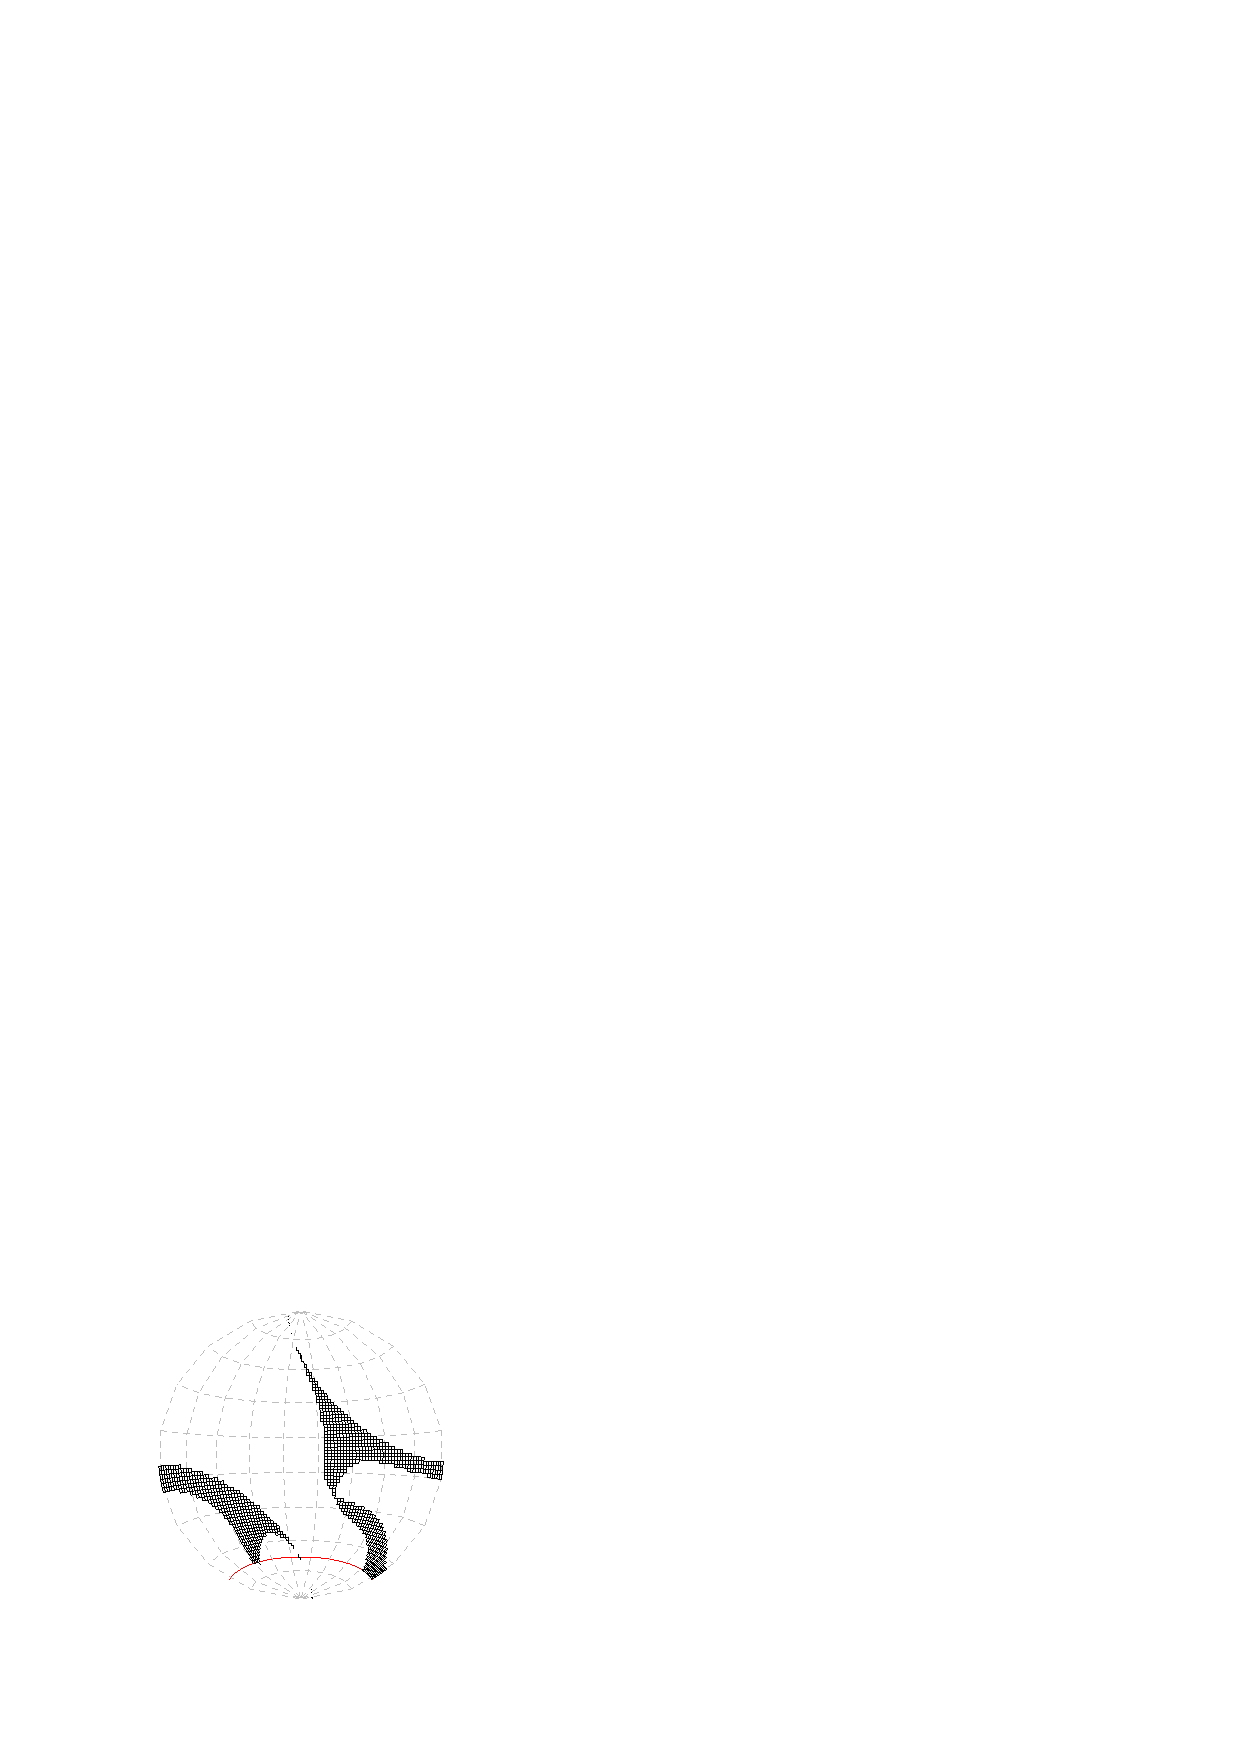
\includegraphics[width=0.5\textwidth]{sphere.pdf}
\caption{Черным показаны направления, в которых можно встретить точку CP-поверхности, если начинать от порождающей ее точки (направления, в которых подынтегральное выражение в \eqref{eq:CPF} не обнуляется). Направление вниз --- направление на центр звезды, направление вверх --- от звезды. Показано только одно полушарие, так как поверхность симметрична относительно плоскости, в которой лежат ось симметрии и точка, ее порождающая. Красной кривой ограничена часть направлений, занимаемая звездой.}
\label{fig:CPmap}
\end{figure}

\newpage

\subsection{Расчет градиента скорости}

Для расчета оптической толщины необходимо знать градиент скорости в сопутствующей системе координат в произвольном направлении: $|\vec{\nabla} (\vec{v}\vec{n})\vec{n}|$. Так как мы работаем в сферической системе координат, необходимо учитывать ее криволинейность, вследствие которой постоянный в пространстве вектор $\vec{n}$ будет непостоянным. Запишем его в сферической системе координат.

\[
\vec{n} = \cos(\alpha)\hat{r} + \frac{1}{r}\sin(\alpha)\cos(\beta)\hat{\theta} + \frac{1}{r\sin\theta}\sin(\alpha)\sin(\beta)\hat{\phi},
\] 
где $\alpha$ --- угол между векторами $\vec{r}$ и $\vec{n}$, а $\beta$ --- угол между проекцией $\vec{n}$ на плоскость, содержащую $\hat{\theta}$ и $\hat{\phi}$, и $\hat{\theta}$. Распишем скалярное произведение:
\[
\vec{v}\vec{n} = vn^r + r^2 u n^\theta.
\]

Далее необходимо вычислить необходимые производные $\vec{n}$. Их можно получить с помощью известного условия, что ковариантная производная постоянного вектора равна нулю 

\[
\nabla_l\ n^m = \frac{\partial n^m}{\partial x^l} + \Gamma^m_{kl} n^k = 0 \Rightarrow \frac{\partial n^m}{\partial x^l} = -\Gamma^m_{kl} n^k.
\]

Здесь по повторным индексам производится суммирование, в котором они пробегают по буквам $r,\theta,\phi$, а $x^r, x^\theta, x^\phi$ --- это просто $r, \theta, \phi$. Так как символы Кристоффеля $\Gamma^m_{kl}$ для сферической системы координат известны, можно записать необходимые нам производные:

\[
\begin{aligned}
\frac{\partial n^\theta}{\partial r} = -\frac{1}{r}n^\theta, \qquad \frac{\partial n^\theta}{\partial \theta} &= -\frac{1}{r}n^r , \qquad \frac{\partial n^\theta}{\partial \phi} = \sin\theta\cos\theta\ n^\phi \\
\frac{\partial n^r}{\partial\theta} &= rn^\theta, \qquad \frac{\partial n^r}{\partial \phi} = r\sin^2\theta\ n^\phi. \\
\end{aligned}
\]

Подставив все, получаем выражение

\begin{align} \label{eq:vecgrad}
\vec{\nabla}(\vec{v}\vec{n})\vec{n} & = \frac{\partial v}{\partial r}\cos^2(\alpha) + \frac{1}{r}\frac{\partial v}{\partial \theta}\cos(\alpha)\sin(\alpha)\cos(\beta) + \frac{v}{r}\sin^2(\alpha) + \nonumber \\
& + \frac{\partial u}{\partial r} \cos(\alpha)\sin(\alpha)\cos(\beta) + \frac{1}{r}\frac{\partial u}{\partial \theta} \sin^2(\alpha)\cos^2(\beta) - \nonumber \\
& - \frac{u}{r}\left(\cos(\alpha)\sin(\alpha)\cos(\beta) - \cot\theta\sin^2(\alpha)\sin^2(\beta)\right).
\end{align}

Если предположить, что движение радиально симметричное ($u = 0$, $\partial v/\partial \theta = 0$), то выражение \eqref{eq:vecgrad} упрощается до известного

\[
\vec{\nabla}(\vec{v}\vec{n})\vec{n} = \frac{\partial v}{\partial r}\cos^2(\alpha) + \frac{v}{r}\sin^2(\alpha).
\] 

\section{Решение уравнения переноса}
\subsection{Ориентация магнитосферы}

Мы рассматриваем возможность отклонения оси магнитосферы от оси вращения звезды. Есть основания предполагать, что такая ситуация встречается у звезд Т Тельца довольно часто (см. например Аленкар и др. \cite{alencar18}). Для того, чтобы было проще моделировать вращательную модуляцию спектральных линий, мы задаем положение магнитосферы при помощи трех углов: угол наклона оси вращения звезды к лучу зрения $i$, отклонение оси магнитосферы от оси вращения $\alpha$, а также фазовый угол вращения $\psi$.

Для расчетов используется декартова система координат с осью Z совпадающей с лучом зрения. Для удобства, ось Y направляется так, чтобы плоскость YZ содержала ось магнитосферы. В такой системе координат положение магнитосферы задается одним углом $\theta$ между осью магнитосферы и лучом зрения, косинус которого равен

\begin{equation} \label{eq:costet}
\cos(\theta) = \cos(i)\cos(\alpha) + \sin(i)\sin(\alpha)\cos(\psi).
\end{equation}

\subsubsection{Вращение магнитосферы}

Для учета вращения магнитосферы необходимо знать направление оси вращения $\vec{a}$. В принятой системе координат этот вектор имеет вид

\begin{align} \label{eq:rotaxis}
a_\text{x} & = \frac{\sin(i)\sin(\alpha)\sin(\psi)}{\sin(\theta)}, \nonumber \\ 
a_\text{y} & = \frac{\sin(i)(\cos(\alpha)\sin(i) - \cos(i)\sin(\alpha)\cos(\psi))}{\sin(\theta)}, \nonumber \\ 
a_\text{z} & = \cos(i).
\end{align}

Тогда можно записать лучевую скорость движения газа в магнитосфере как

\begin{equation} \label{eq:vz}
v_\text{z} = v_\text{zmotion} + v_\text{zrot}, 
\end{equation}
где $v_\text{zmotion}$ --- скорость движения газа (определяемая \eqref{eq:velabs}, \eqref{eq:velvec}), а $v_\text{zrot}$ определяется выражением

\begin{equation} \label{eq:vzrot}
v_\text{zrot} = \frac{v_\text{eq}}{R_\star}(a_\text{x}y - a_\text{y}x),
\end{equation}
где $v_\text{eq}$ --- скорость вращения звезды на экваторе.

\subsection{Расчет профиля линии}


Интенсивность в линии определяется формулой

\begin{equation} \label{eq:profmain}
I_{\nu} = \int \limits_{S} I_{xy}(\nu) dS,
\end{equation}
где $S$ - площадь проекции области на картинную плоскость, а $I_\nu$ - интенсивность излучения в линии перехода $u \rightarrow l$ на частоте $\nu$ 

Рассмотрим $I_{xy}$:
\begin{equation} \label{eq:profproj}
I_{xy}(\nu) = \int \limits_{z_0}^{z_k} S_{ul}(z)k_{lu}(\nu,z)e^{-\tau(\nu,z)}dz,
\end{equation}
\begin{equation} \label{eq:profdepth}
\tau(\nu,z) = \int \limits_z^{z_k} k_{lu}(\nu,z')dz',
\end{equation}
\begin{equation} \label{eq:profsource}
S_{ul}(z) = \frac{2h\nu_0^3}{c^2}\left(\frac{n_l}{n_u} \frac{g_u}{g_l} - 1 \right)^{-1},
\end{equation}
\begin{equation} \label{eq:profabsorb}
k_{lu}(\nu,z) = 0.02654f_{lu}\alpha(\nu, z)n_l\left(1 - \frac{g_l}{g_u}\frac{n_u}{n_l}\right),
\end{equation}
\begin{equation} \label{eq:profabsprof}
\alpha(\nu, z) = \frac{1}{\sqrt{\pi} \Delta\nu_D} \exp\left( -\left[ \frac{\nu - \nu_0}{\Delta\nu_D} - \frac{v_z(z)}{v_t}\right]^2\right),
\end{equation}
где $S_{ul}(z)$ - функция источника, $k_{lu}(\nu, z)$ - коэффициент поглощения, $\nu_0$ - центральная частота линии перехода $l \rightarrow u$, $v_t$ - тепловая скорость, $\Delta\nu_D$ - доплеровская ширина линии, $v_z(z)$ - лучевая скорость вещества.

Для линии Н$\alpha$ вместо доплеровского профиля в \eqref{eq:profabsprof} использовался фойгтовский профиль $H(a, x)$:

\begin{equation} \label{eq:profabsfoigt}
\alpha(\nu, z) = \frac{1}{\sqrt{\pi} \Delta\nu_D}\ H\left(\frac{\delta}{\Delta\lambda_D},\ \left[ \frac{\nu - \nu_0}{\Delta\nu_D} - \frac{v_z(z)}{v_t}\right]\right),
\end{equation}
где 
\begin{equation} \label{eq:foigtcoef}
\Delta\lambda_D = \Delta\nu_D\frac{c}{\nu_0^2},\ \delta = C_{\text{rad}}\ + \ 
 C_{\text{vdW}}\ \frac{n_{\text{HI}}}{10^{16}}\left(\frac{T}{5000 \text{K}}\right)^{0.3} +\ 
 C_{\text{Stark}}\ \frac{n_e}{10^{12}}\ + \ C_{\text{res}}\ \frac{n_\text{HI}}{10^{16}},
\end{equation}
где коэффициенты $C_\text{rad}$, $C_\text{vdW}$, $C_\text{Stark}$ и $C_\text{res}$ взяты из работы \cite{luttermoser92}. Для расчета $H(a, x)$ использовались разложения в ряд и программа из работы \cite{humlicek82}.

Излучение в континууме задается формулой Планка:

\begin{equation} \label{eq:profcont}
I_c = \frac{2h\nu^3}{c^2}\frac{1}{\exp\left(\frac{h\nu}{k_bT_\star}\right)-1},
\end{equation}
где $T_\star$ - эффективная температура звезды. Теперь можно рассчитать профиль $r_{\nu}$

\begin{equation} \label{eq:profnorm}
r_{\nu} = \frac{I_\nu + I_{\tau}(\nu)}{I_c \pi R_\star^2},
\end{equation}
где $I_{\tau}$ учитывает поглощение излучения звезды в магнитосфере:

\begin{equation} \label{eq:absorbprof}
I_{\tau}(\nu) = \int \limits_{S_\star} I_c e^{-\tau} dS,
\end{equation}
где $S_\star$ - проекция звезды на картинную плоскость, а $\tau$ - оптическая толщина на всем луче.

\section{Результаты}
Для расчетов автором были написаны 2 программы на языке Фортран: одна --- для решения системы уравнений стационарности, основанная на программе из работы \cite{katysheva80}, в которую были введены дополнительные радиационные члены, учитывающие нелокальное взаимодействие, другая --- для расчета профиля линии при различных ориентациях магнитосферы. Первая из них затем была подключена к программе на языке Python, чтобы рассчитывать температурный режим способом, описанном в работе Хартманна и др. \cite{hartmann94}. В таблице \ref{tab:par} перечислены необходимые параметры для расчета одного профиля. Значения некоторых из них мы не меняли в процессе расчетов. Эти значения также указаны в таблице.

\begin{table}[hb]
\centering
\begin{tabular}[c]{|l l c|}
	% \hline
	\multicolumn{2}{c}{\textbf{Параметры магнитосферы}} \\
	\hline
	$r_\text{mi}$ & Внутренний радиус магнитосферы & $2.2 R_\star$\\
	\hline
	$r_\text{mo}$ & Внешний радиус магнитосферы & $3.0 R_\star$\\
	\hline
	$\dot{M}$ & Темп аккреции & \\
	\hline
	$T_\text{max}$ & Максимальная температура в магнитосфере без учета горячей области & \\
	\hline
	$d_\text{hot}$ & Размер горячей области у поверхности звезды & \\
	\hline
	$T_\text{hot}$ & Прибавка к температуре в горячей области & \\
	\hline
	\multicolumn{2}{c}{\textbf{Параметры звезды}} \\
	\hline
	$R_\star $ & Радиус звезды & $2 R_\odot$ \\
	\hline
	$M_\star $ & Масса звезды & $0.8 M_\odot$ \\
	\hline
	$T_\star $ & Температура звезды & $4000\text{K} $ \\
	\hline
	$v_\text{eq}$ & Скорость вращения звезды на экваторе & \\
	\hline
	\multicolumn{2}{c}{\textbf{Параметры ориентации оси магнитосферы}} \\
	\hline
	$i$ & Угол наклона оси вращения звезды к лучу зрения & \\
	\hline
	$\alpha$ & Угол наклона оси магнитосферы к оси вращения звезды & \\
	\hline
	$\psi$ & Фаза вращения звезды & \\
	\hline
\end{tabular}
\caption{Параметры модели}
\label{tab:par}
\end{table}

\subsection{Решение системы уравнений стационарности}

На рис. \ref{fig:grid} показана сетка, в каждой точке которой решалась система уравнений стационарности. На рис. \ref{fig:grad} показано поведение градиента скорости \eqref{eq:vecgrad} на каждой линии тока с рис. \ref{fig:grid} в зависимости от расстояния до центра звезды в ее радиусах.
% \pagebreak
\begin{figure}[!h]
\centering
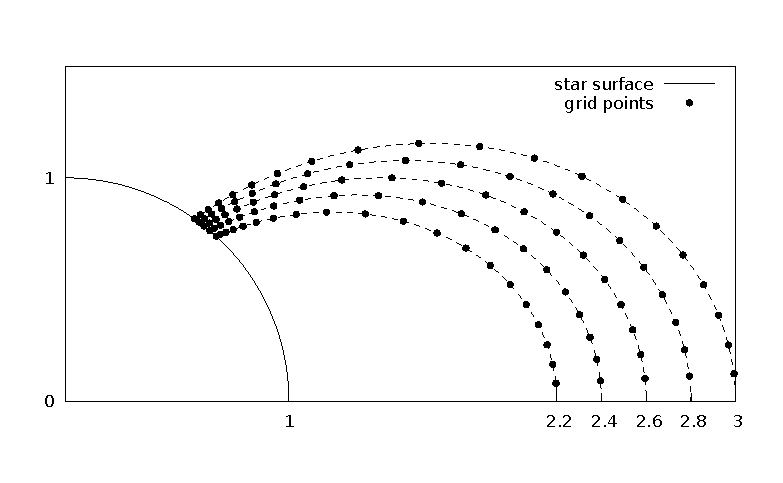
\includegraphics[width=0.8\textwidth]{grid.eps}
\caption{Показаны точки сетки, в которых решалась система уравнений стационарности. Пунктирными линиями показаны пять линий тока. Также показана поверхность звезды.}
\label{fig:grid}
\end{figure}
% \newpage
\begin{figure}[!h]
\centering
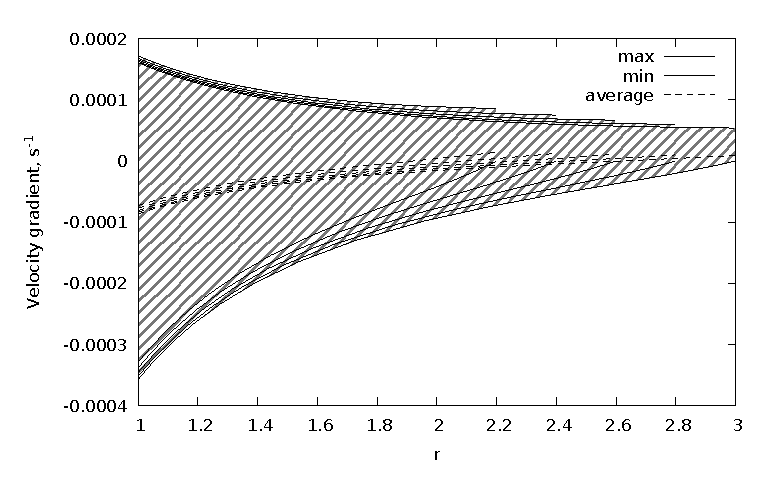
\includegraphics[width=0.8\textwidth]{grad.eps}
\caption{Разброс градиента скорости по направлению \eqref{eq:vecgrad} в магнитосфере. Показаны максимальный, минимальный и средний по направлениям градиент.}
\label{fig:grad}
\end{figure}
% \newpage

\FloatBarrier

Рис. \ref{fig:TeNe} и \ref{fig:N1N2} демонстрируют поведение температуры, концентрации электронов, населенностей первого и второго уровня в магнитосфере с $\dot{M} = 10^{-7}\ \text{M}_\odot/$год и $T_\text{max} = 7500\ \text{K}$ в зависимости от расстояния до центра звезды в ее радиусах. Нелокальное взаимодействие практически не влияет на вид зависимостей, однако оно немного поднимает значения населенностей третьего и выше лежащих уровней вблизи начала линий тока ($R \approx r_\text{m}$), так как позволяет фотонам, порожденным в более горячих областях, поглотится в более холодных.


\begin{figure}[!h]
\centering
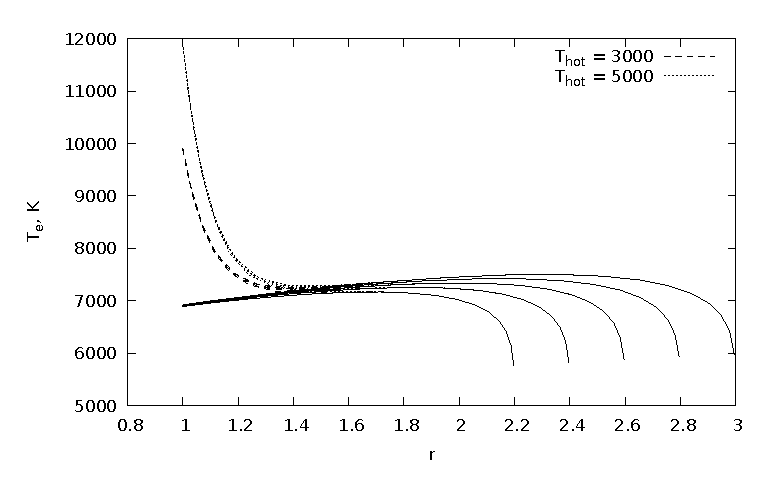
\includegraphics[width=0.8\textwidth]{T_e.eps}
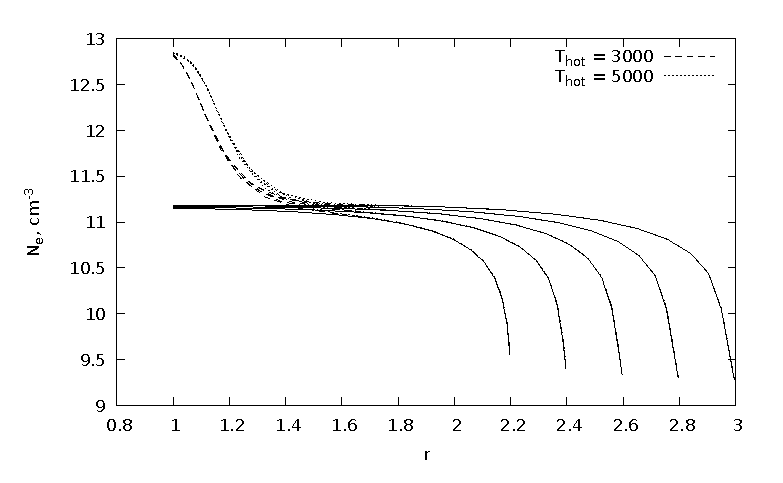
\includegraphics[width=0.8\textwidth]{N_e.eps}
\caption{Температура ($T_\text{e}$) и электронная концентрация ($N_\text{e}$) в магнитосфере. Штрихом и пунктиром показан вклад горячей области с $d_\text{hot} = 0.1 R_\star$}
\label{fig:TeNe}
\end{figure}

\begin{figure}[!h]
\centering
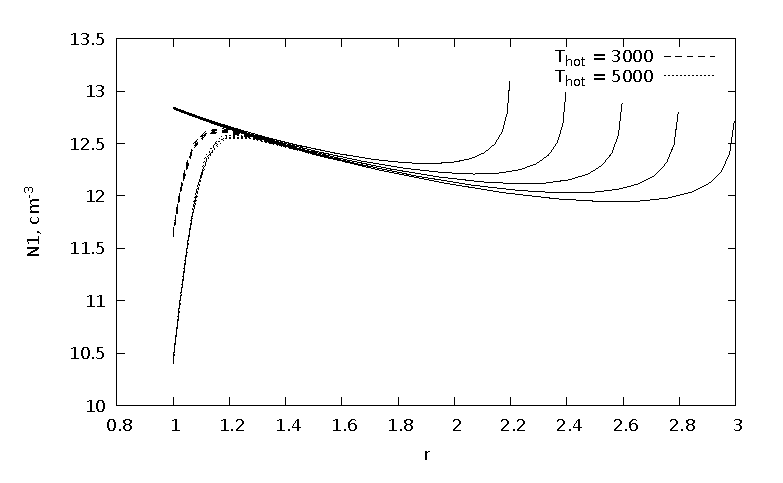
\includegraphics[width=0.9\textwidth]{N1.eps}
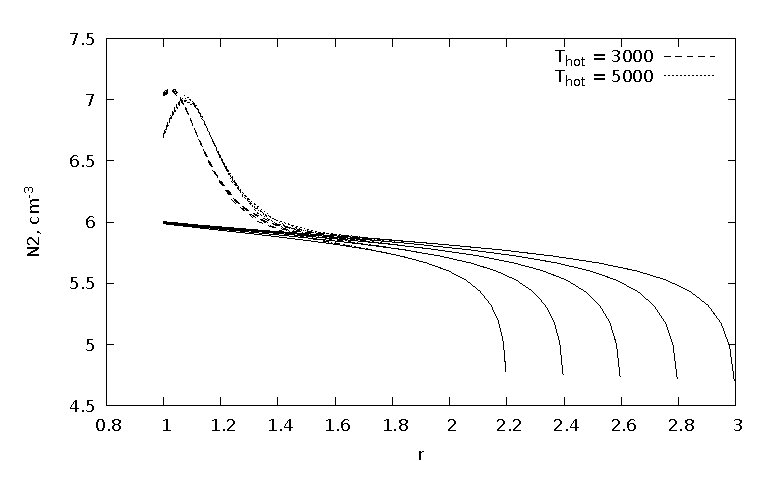
\includegraphics[width=0.9\textwidth]{N2.eps}
\caption{Населенности первого и второго уровня в магнитосфере. Штрихом и пунктиром показан вклад горячей области с $d_\text{hot} = 0.1 R_\star$}
\label{fig:N1N2}
\end{figure}
\FloatBarrier
% \pagebreak
\subsection{Профили водородных линий без учета вращения магнитосферы}

На рис. \ref{fig:Ha}-\ref{fig:Brg} показаны профили линий $\text{H}\alpha$, $\text{H}\beta$, $\text{H}\gamma$ и $\text{Br}\gamma$. При этом угол $\alpha$ равен нулю, и следовательно ось магнитосферы совпадает с осью вращения. Скорость вращения $v_\text{eq}$ принималась равной нулю. На рисунках также продемонстрирован вклад горячей области с $d_\text{hot} = 0.1 R_\star$. Можно заметить, что двукомпонентность линий бальмеровской серии наблюдается на маленьких углах наклона при больших темпах аккреции, а на больших углах при меньших темпах аккреции.

 


\begin{figure}[h]
\centering
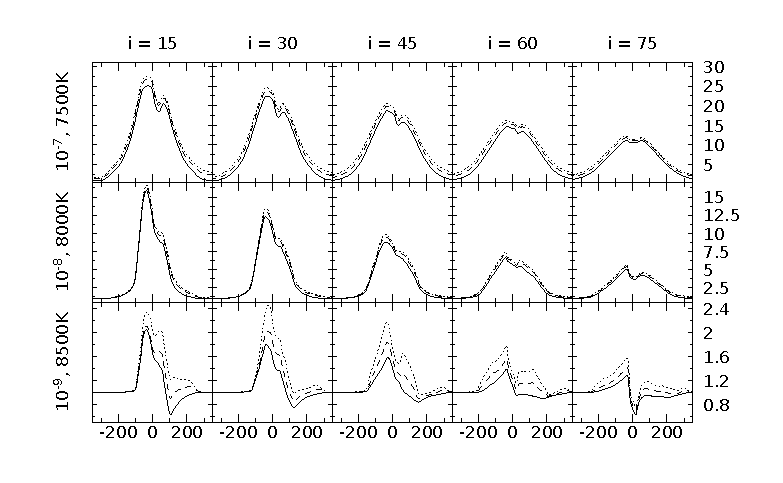
\includegraphics[width=\textwidth]{hot_5_Ha.eps}
\caption{Профили линии $\text{H}\alpha$ для различных углов, темпов аккреции и температур. Слева подписаны темп аккреции $\dot{M}$ в $\text{M}_\odot$/год и температура $T_\text{max}$, сверху --- угол наклона оси магнитосферы к лучу зрения в градусах. Штрихом нанесены профили в моделях с дополнительным нагревом: $T_\text{hot} = 3000\ \text{K}$, $d_\text{hot} = 0.1$. Пунктиром: $T_\text{hot} = 5000\ \text{K}$, $d_\text{hot} = 0.1$.}
\label{fig:Ha}
\end{figure}
% \pagebreak
% \pagebreak
\begin{figure}[h]
\centering
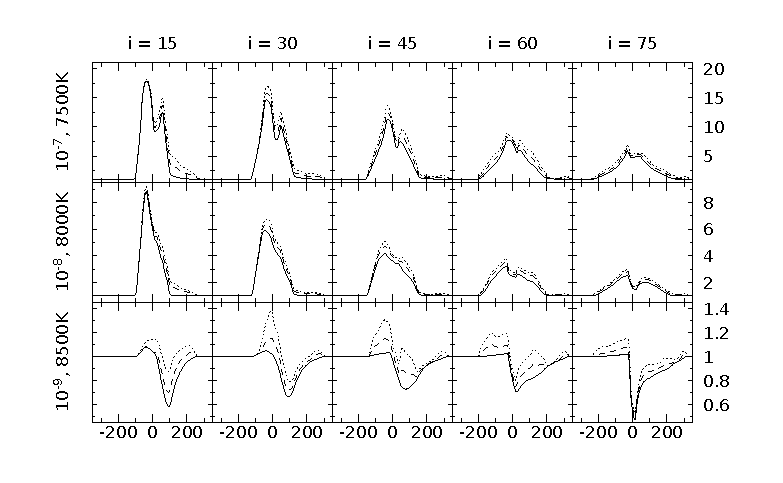
\includegraphics[width=\textwidth]{hot_5_Hb.eps}
\caption{Профили линии $\text{H}\beta$ для различных углов, темпов аккреции и температур. Слева подписаны темп аккреции $\dot{M}$ в $\text{M}_\odot$/год и температура $T_\text{max}$, сверху --- угол наклона оси магнитосферы к лучу зрения в градусах. Штрихом нанесены профили в моделях с дополнительным нагревом: $T_\text{hot} = 3000\ \text{K}$, $d_\text{hot} = 0.1$. Пунктиром: $T_\text{hot} = 5000\ \text{K}$, $d_\text{hot} = 0.1$.}
\label{fig:Hb}
\end{figure}

\begin{figure}[h]
\centering
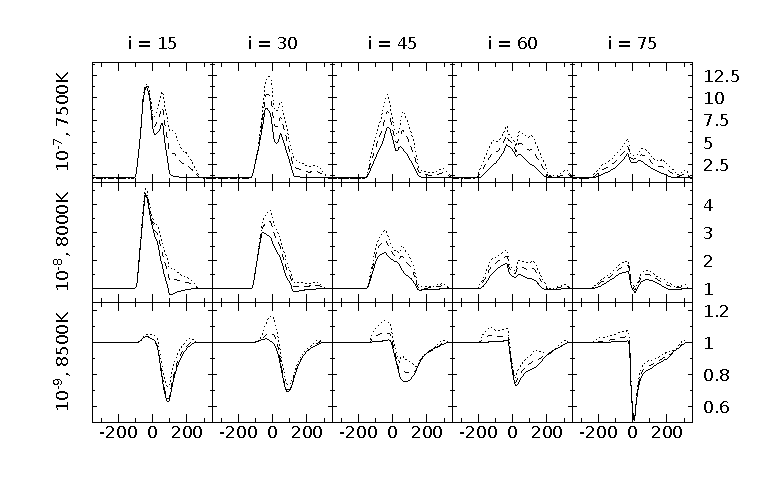
\includegraphics[width=\textwidth]{hot_5_Hg.eps}
\caption{Профили линии $\text{H}\gamma$ для различных углов, темпов аккреции и температур. Слева подписаны темп аккреции $\dot{M}$ в $\text{M}_\odot$/год и температура $T_\text{max}$, сверху --- угол наклона оси магнитосферы к лучу зрения в градусах. Штрихом нанесены профили в моделях с дополнительным нагревом: $T_\text{hot} = 3000\ \text{K}$, $d_\text{hot} = 0.1$. Пунктиром: $T_\text{hot} = 5000\ \text{K}$, $d_\text{hot} = 0.1$.}
\label{fig:Hg}
\end{figure}

\begin{figure}[h]
\centering
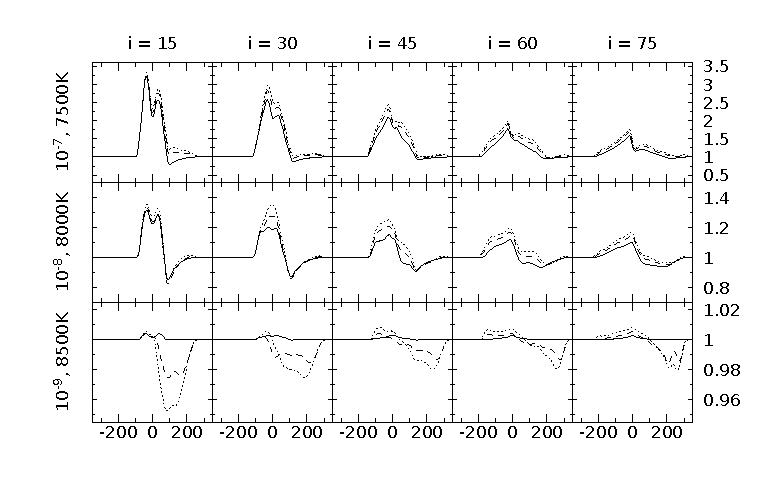
\includegraphics[width=\textwidth]{hot_5_Brg.eps}
\caption{Профили линии $\text{Br}\gamma$ для различных углов, темпов аккреции и температур. Слева подписаны темп аккреции $\dot{M}$ в $\text{M}_\odot$/год и температура $T_\text{max}$, сверху --- угол наклона оси магнитосферы к лучу зрения в градусах. Штрихом нанесены профили в моделях с дополнительным нагревом: $T_\text{hot} = 3000\ \text{K}$, $d_\text{hot} = 0.1$. Пунктиром: $T_\text{hot} = 5000\ \text{K}$, $d_\text{hot} = 0.1$.}
\label{fig:Brg}
\end{figure}
\FloatBarrier

Из результатов видно, что чем больше угол $i$, тем менее интенсивными и более широкими становятся линии. Однако, для малых темпов аккреции с дополнительным нагревом, самые интенсивные профили наблюдаются при $i=30$\degree. Также видно, что двукомпонентность профилей наблюдается на разных углах наклона при разных параметрах модели: при больших темпах аккреции на углах $i$ близких к 0\degree, а при меньших на близких к 90\degree. Дополнительный нагрев магнитосферы приводит к увеличению интенсивности профилей и к достаточно сложным изменениям их формы. Для угла наклона $i=15$\degree\ дополнительный нагрев приводит к увеличение яркости красного крыла профиля. Для углов наклона $i > 30$\degree\ в линиях Н$\beta$ и H$\gamma$ появляется небольшой эмиссионный компонент на скоростях около 300 км/с. В целом вклад дополнительного нагрева более заметен в слабых линиях. 

\subsection{Учет вращения магнитосферы}

В этом разделе демонстрируются эффекты вращения магнитосферы вокруг оси, не совпадающей с ее осью. Основным эффектом является переменность спектральных линий, вызванная наклоном оси магнитосферы к оси вращения на угол $\alpha = 15\text{\degree}$. Скорость вращения звезды на экватаре $v_\text{eq}$ предполагалась равной 15 км/с (среднее значение для звезд типа Т Тельца \cite{petrov03}). Остальные параметры звезды, а также размеры магнитосферы, остаются такими же, как и в предыдущем разделе. При расчете профилей мы не учитывали вклад горячей области. Полученные профили линии H$\beta$ при темпах аккреции $10^{-7}$ и $10^{-8}\ \text{M}_\odot$/год и при температурах 7500 К и 8000 К показаны на рис. \ref{fig:rot7} и \ref{fig:rot8}.

\begin{figure}[h]
\centering
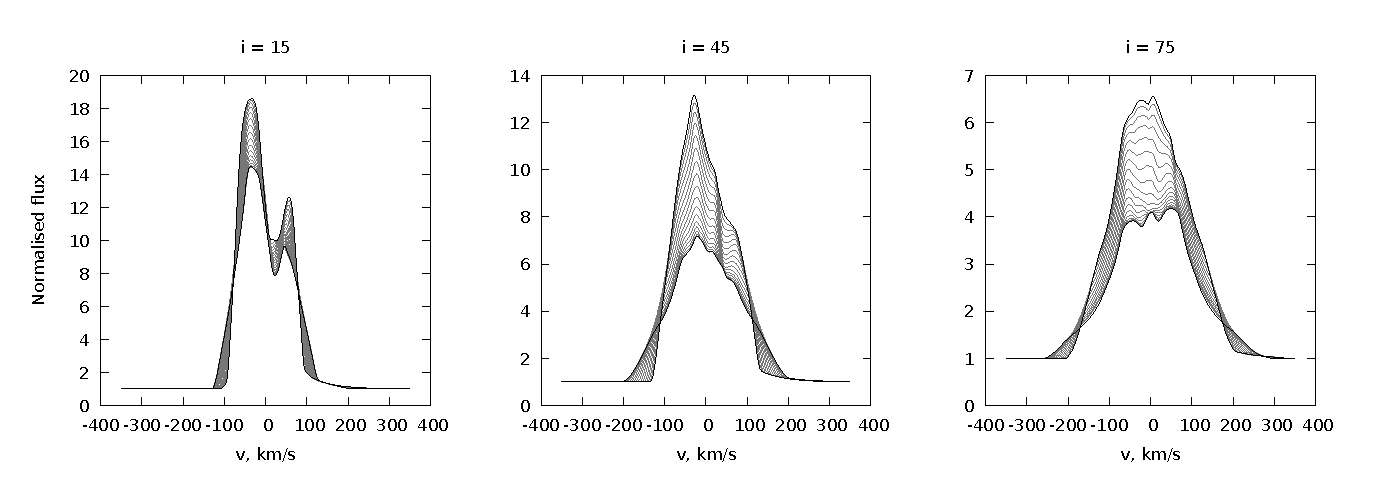
\includegraphics[width=\textwidth]{rot_7.eps}
\caption{Переменность профиля линии H$\beta$ при вращении магнитосферы с $\dot{M} = 10^{-7}\ \text{M}_\odot/$год и $T_\text{max} = 7500\ \text{K}$. Серыми линиями нанесены профили для разных фаз $0$\degree$< \psi < 180$\degree\ с шагом в 10\degree. Черными линиями отмечены крайние фазы $\psi = 0\text{\degree}$ и $\psi = 180\text{\degree}$}
\label{fig:rot7}
\end{figure}

\begin{figure}[h]
\centering
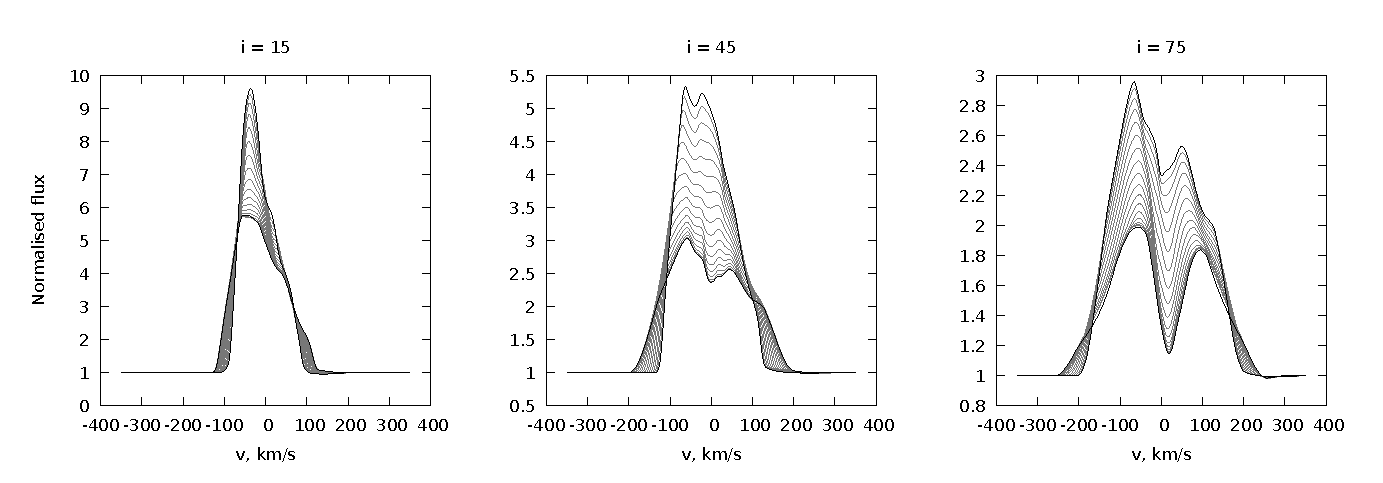
\includegraphics[width=\textwidth]{rot_8.eps}
\caption{Переменность профиля линии H$\beta$ при вращении магнитосферы с $\dot{M} = 10^{-8}\ \text{M}_\odot/$год и $T_\text{max} = 8000\ \text{K}$. Серыми линиями нанесены профили для разных фаз $0$\degree$< \psi < 180$\degree\ с шагом в 10\degree. Черными линиями отмечены крайние фазы $\psi = 0\text{\degree}$ и $\psi = 180\text{\degree}$}
\label{fig:rot8}
\end{figure}

\FloatBarrier

\section{Сравнение с наблюдениями}

В целом удается получить профили, качественно очень похожие на наблюдаемые. Мы не проводили детальной подгонки профилей, и из-за этого значения потоков и некоторые детали профилей не совпадают. На рис. \ref{fig:compprof} сравниваются профили из работы \cite{antoniucci17} и теоретические профили для $i = 45$\degree\ и $\alpha = 0$\degree, параметров звезды и размеров магнитосферы из таблицы \ref{tab:par}, $\dot{M} = 10^{-8}\ \text{M}_\odot/$год и $T_\text{max} = 8000$ K. 

\begin{figure}[h]
\centering
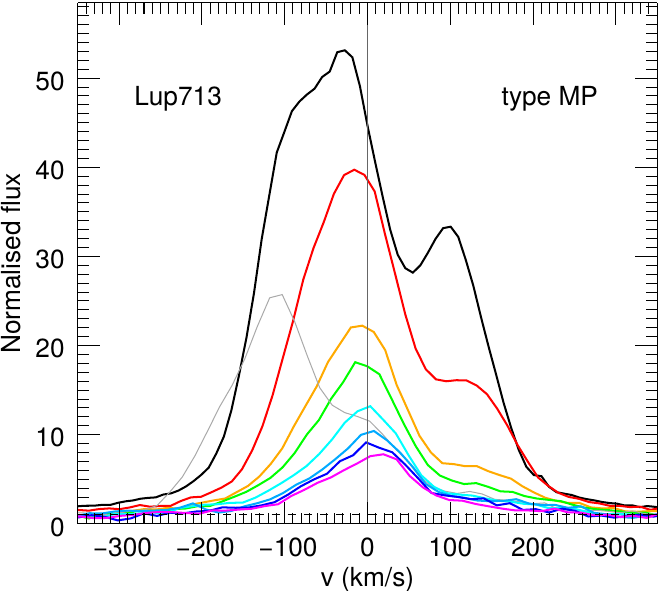
\includegraphics[width=0.45\textwidth]{profiles2.png}
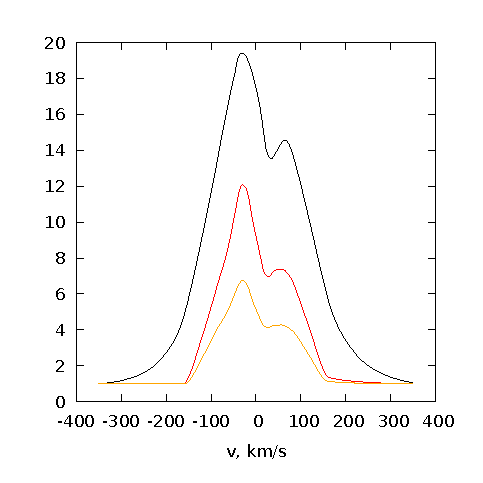
\includegraphics[width=0.4\textwidth]{lookslike45.eps}
\caption{Наблюдаемые (слева) профили бальмеровских линий из работы \cite{antoniucci17} и похожие на них по форме теоретические профили (справа).}
\label{fig:compprof}
\end{figure} 

\FloatBarrier

Переменность теоретических профилей также качественно согласуется с наблюдаемой. На рис. \ref{fig:compvar} показана наблюдаемая переменность линии Н$\alpha$ из работы \cite{sousa16}, которая похожа на представленную на рис. \ref{fig:rot7} слева (происходит переход от двукомпонентного профиля к треугольному).

\begin{figure}[h]
\centering
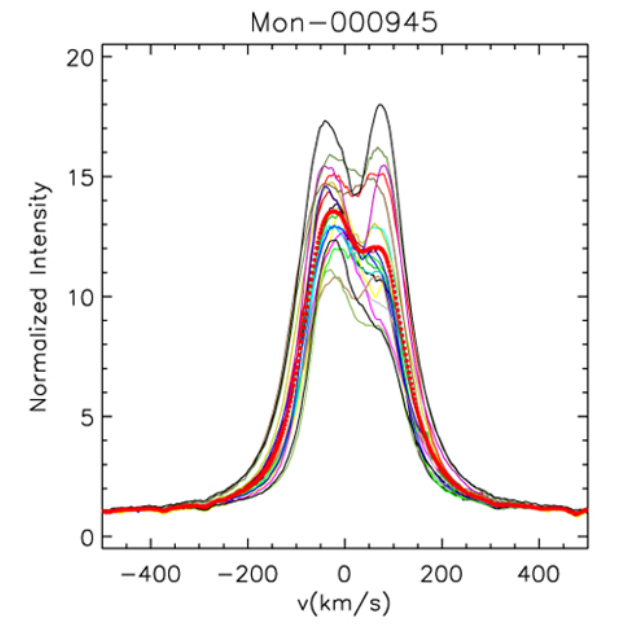
\includegraphics[width=0.5\textwidth]{profilevar.png}
\caption{Наблюдаемая переменность линии H$\alpha$ из работы \cite{sousa16}.}
\label{fig:compvar}
\end{figure} 

\FloatBarrier

\section{Заключение}

Основным результатом данной работы является программная реализация алгоритма, позволяющего моделировать профили магнитосферных линий в спектрах молодых звезд. 
%Эту модель можно использовать вместе с существующими моделями ветров для определения параметров магнитосферы, таких как темп аккреции и температура в ней. 
Полученные профили водородных линий похожи на теоретические профили из работ Хартманна \cite{hartmann94} и Мацеролле \cite{muzerolle01}. Полного совпадения ожидать нельзя, так как модели не совсем идентичны. Сравнение с наблюдениями показало, что теоретические профили хорошо воспроизводят все основные детали наблюдаемых, в спектрах, с преобладающим вкладом излучения магнитосферы. 

Также мы продемонстрировали возможность моделировать наблюдаемую переменность линий вращением магнитосферы, ось которой наклонена относительно оси вращения звезды.

\begin{thebibliography}{99}
% \bibitem{hartmann94}{\it 
% Хартманн и др.} (L. Hartmann, R. Hewett, N. Calvet), Astrophys. J. {\bf 426}, 669 (1994). 

% \bibitem{lima10}{\it Лима и др.} (G.H.R.A. Lima, S.H.P. Alencar, N. Calvet \etal ) Astron. Astrophys. {\bf 522}, A104 (2010)

% \bibitem{hartmann01}{\it Мацеролли и др.} (J. Muzerolle, N. Calvet, L. Hartmann ) Astrophys. J. {\bf 550}, 944 (2001)

% \bibitem{rybicki78}{\it Райбики, Хаммер } (G.B. Rybicki, D.G. Hummer ) Astrophys. J. {\bf 219}, 654 (1978)

% \bibitem{grachev75}{\it Грачев С.И., Гринин В.П.}, Астрофизика {\bf 11}, 20 (1975)

% \bibitem{katysheva80} Катышева Н.А., Гринин В.П., Изв. КрАО, 1980, 62, 52

\bibitem{petrov03} Петров, П.П., Астрофизика, 2003, том 46, No 4, c. 506
\bibitem{hartmann94} Hartmann, L., Hewett, R., \etal, ApJ, 1994, 426, 669
\bibitem{matt05} Matt, S., Pudritz, R.E., ApJL, 2005, 632, L135
\bibitem{muzerolle01} Muzerolle, J., Calvet, N., \etal, ApJ, 2001, 550, 944
\bibitem{lima10} Lima, G.H.R.A., Alencar, S.H.P., \etal, A\&A, 2010, 522, A104
\bibitem{grachev75} Грачев, С.И., Гринин, В.П., Астрофизика, 1975, 11, 20 
\bibitem{rybicki78} Rybicki, G.B., Hummer, D.G., ApJ, 1978, 550, 944
\bibitem{tambovtseva14} Tambovtseva, L.V., Grinin, V.P, \etal, A\&A, 2014, 562, A104
\bibitem{grinin11} Гринин В.П., Tамбовцева, Л.В., АЖ, 2011, том 88, No 8, с. 766
\bibitem{antoniucci17} Antoniucci, S., Nisini, B., \etal, A\&A, 2017, 599, A105
\bibitem{bouvier99} Bouvier, J., Chelli A., \etal, A\&A, 1999, 349, 619
\bibitem{petrov01} Petrov, P.P., Gahm, G.F., \etal, A\&A, 2001, 369, 993
\bibitem{dodin18} Dodin, A., MNRAS, 2018, 475, 4367
\bibitem{lamzin98} Ламзин, С.А., АЖ, 1998, 47, 498
\bibitem{katysheva80} Катышева, Н.А., Гринин, В.П., Изв. КрАО, 1980, 62, 52
\bibitem{alencar18} Alencar, S.H.P., Teixeira, P.S., \etal, A\&A, 2010, 519, A88 
\bibitem{luttermoser92} Luttermoser, D.G., Johnson, H.R., ApJ, 1992, 388, 579
\bibitem{humlicek82} Humlicek, J., J. Quant. Spectrosc. Radiat. Transfer, 1982, Vol. 27, No. 4, P. 437 
% \bibitem{kenyon95} Kenyon, S.J., Hartmann L., 1995, ApJS, 101, 117
% \bibitem{palla99} Palla, F., Stahler, S. W., 1999, ApJ, 525, 772
% \bibitem{dullemond07} Dullemond, C.P., et al., 2007, Protostars and Planets V (Tuscon,AZ: Univ. Arizona Press),555
% \bibitem{krull99} Johns-Krull, C.M., et al. A.1999, ApJL, 510, L41
% \bibitem{gunther13} Gunther, H. M. 2013, AN, 334, 67
\bibitem{sousa16} Sousa, A.P., Alencar, S.H.P., \etal, A\&A, 2016, 586, A47
% \bibitem{cranmer09} Cranmer, S. R.: 2009, ApJ 706, 824
% \bibitem{matt07} Matt, S. \& Pudritz, R. E.: 2007, in IAU Symposium, Vol. 243, p. 299
% \bibitem{herbst94} Herbst, W. et al. 1994,AJ, 108, 1906
% \bibitem{petrov99} Petrov, P.P. et al. 1999, A\& ;A, 341, 553

\end{thebibliography}
\end{document}